%%%%%%%%%%%%%%%%%%%%%%%%%%%%%%%%%%%%%%%%%%%%%%%%%%%%%%%%%%%%%%%%
%                                                              %
%          GuIT - Gruppo Italiano Utilizzatori di TeX          %
%                                                              %
%          M. Himmelmann, E. Vavassori, F. Busdraghi           %
%                                                              %
%           ---  Introduzione al mondo di LaTeX  ---           %
%                         Versione 1.1                         %
%                                                              %
%     Questo materiale è rilasciato sotto licenza CCPL 2.5     % 
% Consultare la documentazione allegata per maggiori dettagli  %
%                                                              %
%%%%%%%%%%%%%%%%%%%%%%%%%%%%%%%%%%%%%%%%%%%%%%%%%%%%%%%%%%%%%%%%

% vim:sts=2:ts=2:tw=70
\documentclass[svgnames,%
	ucs,% Serve per l'encoding UTF8
	pdftex]{guitbeamer}
\usepackage[utf8x]{inputenc}
\graphicspath{{img/}}

\usepackage{setspace,textcomp}

% pacchetti necessari per le slide
\usepackage{rotating}

% esempio del testo rotante
\newcounter{wang}
\newlength{\wangspace}
\newsavebox{\wangtext}
\newcommand{\wheel}[1]{%
	\savebox{\wangtext}{#1}%
	\settowidth{\wangspace}{#1}
	\addtolength{\wangspace}{1cm}
	\centerline{%
		\rule{0pt}{\wangspace}%
		\rule[-\wangspace]{0pt}{%
			\wangspace}%
		\setcounter{wang}{-180}%
		\whiledo{%
			\value{wang} < 180}{%
			\rlap{\begin{rotate}{%
				\value{wang}}
				\rule{1cm}{0pt}#1%
			      \end{rotate}}
			\addtocounter{wang}{10}}}}
\singlespacing

% Titolo del corso, autore, data
\title{Introduzione al mondo di \LaTeX}
\author[Maurizio W.\,Himmelmann]{Maurizio W.\,Himmelmann}
\date{12 dicembre 2008} % qui ci va anche l'evento

% Si comincia :)
\begin{document}


% Pagina del titolo
\frame{\titlepage}
%-----------------------------------------------------------
%--------------------------------------------------- SLIDE -
\begin{frame}
  \frametitle{Guide consigliate}
	\begin{thebibliography}{Fer66}
		\bibitem [GC05]{CAS}
			Caschili, Massimo.
			\newblock\textit{Semplici Figure con l'Ambiente Picture}.
			\newblock  Ars\TeX nica, 1/2006
		\bibitem [TT04]{TAN}
			Tantau, Till.
			\newblock\textit{User's Guide to the Beamer Class}.
			\newblock
			{\small\url{http://latex-beamer.sourceforce.net/}}
	\end{thebibliography}
\end{frame}
%-----------------------------------------------------------
%--------------------------------------------------- SLIDE -
\begin{frame}
  \frametitle{Piano della presentazione}
  \tableofcontents
\end{frame}
%-----------------------------------------------------------
%------------------------------------------------- SECTION -
\section{Figure ed immagini}
%-----------------------------------------------------------
%--------------------------------------------------- SLIDE -
\begin{frame}
  \frametitle{Figure ed immagini}
	\LaTeX prevede sia la possibilit\`a di produrre figure per proprio conto che di inserire figure esterne prodotte da altri programmi. In quest'ultimo caso si segue una metodica diversa dai comuni editor WYSIWYG:
	\begin{itemize}
		\item le figure rimangono in \emph{file separati}, cio\`e la figura non va ``incollata'' nel documento ma \`e sufficiente scrivere un collegamento ad essa.\\
	\end{itemize}
	Risulta quindi conveniente:
	\begin{itemize}
		\item creare nella directory di lavoro una cartella \LCmd[]{img}
		\item salvare in questa directory tutti i file da inserire nel nostro documento finale.
	\end{itemize}
\end{frame}
%-----------------------------------------------------------
%--------------------------------------------------- SLIDE -
\begin{frame}
  \frametitle{Vantaggi e svantaggi}
	Vantaggi:
	\begin{itemize}
		\item se i contenuti delle figure vegono cambiati \`e sufficiente sostituire i file e ricompilare. Il nuovo documento generato avr\`a tutte le figure aggiornate
		\item la procedura \`e molto stabile e non crea brutte sorprese
	\end{itemize}
	Svantaggi:
	\begin{itemize}
		\item serve un minimo di esperienza per una piena padronanza del meccanismo 
		\item richiede l'uso di programmi in grado di lavorare in modo sinergico con \LaTeX
	\end{itemize}
\end{frame}
%-----------------------------------------------------------
%--------------------------------------------------- SLIDE -
\begin{frame}
  \frametitle{Estensioni supportate}
	Esistono due principali tipi di figure:\\
  \bigskip
	Vettoriali (generalmente indicate per i grafici)
	\begin{itemize}
		\item \Lopt{.pdf} (portable document file) 
		\item \Lopt{.eps} (encapsulated postcript) 
		\item \Lopt{.ps} (postcript) 
	\end{itemize}
  \bigskip
	Bitmap (generalmente indicate per immagini)
	\begin{itemize}
		\item \Lopt{.png} (portable network graphics)
		\item \Lopt{.jpeg} o \Lopt{.jpg} (joint photographic experts group) 
		\item \Lopt{.tiff} o \Lopt{.tif} (tagged image file format) 
	\end{itemize}
\end{frame}
%-----------------------------------------------------------
%--------------------------------------------------- SLIDE -
\begin{frame}
  \frametitle{Estensioni supportate}
	pdf\LaTeX\ supporta direttamente file con le seguenti estensioni:
	\begin{itemize}
		\item \Lopt{.pdf} (portable document file) 
		\item \Lopt{.png} (portable network graphics)
		\item \Lopt{.jpeg} (encapsulated postcript) 
		\item \Lopt{.tiff} (tagged image file format) 
	\end{itemize}
  \medskip
	Gli altri formati (\LCmd[]{.eps}, \LCmd[]{.ps}) andranno convertiti in \LCmd[]{.pdf} se non si vorr\`a usare un differente compilatore.
\end{frame}
%-----------------------------------------------------------
%--------------------------------------------------- SLIDE -
\subsection{Il pacchetto graphicx}
%-----------------------------------------------------------
%--------------------------------------------------- SLIDE -
\begin{frame}
  \frametitle{L'oggetto del nostro gioco}
	\begin{center}
		
\includegraphics[]{lion}\\
		\texttt{lion.png}
	\end{center}
  \onslide<2->
	\begin{block}{Attenzione!}
		\`E necessario caricare il pacchetto \Lsty{graphicx} (con l'opzione \LCmd[]{pdftex} nel caso in cui si usi pdf\LaTeX\ come compilatore)
	\end{block}
\end{frame}
%-----------------------------------------------------------
%--------------------------------------------------- SLIDE -
\begin{frame}
  \frametitle{Il pachetto \texttt{graphicx}}
	\begin{LaTeXcode}
		\\includegraphics\{lion\}
	\end{LaTeXcode}
	\begin{center}
		
\includegraphics[]{lion}
	\end{center}
  \onslide<2->
	\begin{block}{Il bello di \LaTeX}
		\`E consigliabile non specificare l'estensione del file 
	\end{block}
\end{frame}
%-----------------------------------------------------------
%--------------------------------------------------- SLIDE -
\begin{frame}
  \frametitle{Il pachetto \texttt{graphicx}}
	\`E possibile indicare nel preambolo una specifica cartella dove sono contenute tutte le figure utilizzate all'interno del documento 
	\begin{LaTeXcode}
		\alert{\\graphicspath\{\{}<path>\alert{\}\}}
	\end{LaTeXcode}
	Alternativamente \`e possibile specificarlo singolarmente all'interno di ogni singolo \LCmd{includegraphics}
	\begin{LaTeXcode}
		\\includegraphics\{\alert{<path>}lion\}
	\end{LaTeXcode}
\end{frame}
%-----------------------------------------------------------
%--------------------------------------------------- SLIDE -
\begin{frame}
  \frametitle{Un esempio vale pi\`u di mille figure}
	\begin{center}
		\alert{\texttt{esempio\_4\_1.tex}}
	\end{center}
\end{frame}
%-----------------------------------------------------------
%--------------------------------------------------- SLIDE -
\begin{frame}
  \frametitle{Il pachetto \texttt{graphicx}}
	\begin{LaTeXcode}
		\alert{\\fbox\{}\\includegraphics\{lion\}\alert{\}}
	\end{LaTeXcode}
	\begin{center}
		\fbox{
\includegraphics[]{lion}}
	\end{center}
\end{frame}
%-----------------------------------------------------------
%--------------------------------------------------- SLIDE -
\begin{frame}
  \frametitle{Il pachetto \texttt{graphicx}}
	\begin{LaTeXcode}
		\\includegraphics\alert{[scale=0.5]}\{lion\}
	\end{LaTeXcode}
	\begin{center}
		
\includegraphics[scale=0.5]{lion}
	\end{center}
\end{frame}
%-----------------------------------------------------------
%--------------------------------------------------- SLIDE -
\begin{frame}
  \frametitle{Il pachetto \texttt{graphicx}}
	\begin{LaTeXcode}
		\\includegraphics\alert{[scale=1.5]}\{lion\}
	\end{LaTeXcode}
	\begin{center}
		
\includegraphics[scale=1.5]{lion}
	\end{center}
\end{frame}
%-----------------------------------------------------------
%--------------------------------------------------- SLIDE -
\begin{frame}
  \frametitle{Il pachetto \texttt{graphicx}}
	\begin{LaTeXcode}
		\\includegraphics\alert{[width=20mm]}\{lion\}
	\end{LaTeXcode}
	\begin{center}
		
\includegraphics[width=20mm]{lion}
	\end{center}
\end{frame}
%-----------------------------------------------------------
%--------------------------------------------------- SLIDE -
\begin{frame}
  \frametitle{Il pachetto \texttt{graphicx}}
	\begin{LaTeXcode}
		\\includegraphics\alert{[width=20mm, height=40mm]}\{lion\}
	\end{LaTeXcode}
	\begin{center}
		
\includegraphics[width=20mm, height=40mm]{lion}
	\end{center}
\end{frame}
%-----------------------------------------------------------
%--------------------------------------------------- SLIDE -
\begin{frame}
  \frametitle{Il pachetto \texttt{graphicx}}
	\begin{LaTeXcode}
		\\includegraphics\alert{[width=20mm, height=40mm,}\n
		\alert{keepaspectratio]}\{lion\}
	\end{LaTeXcode}
	\begin{center}
		
\includegraphics[width=20mm, height=40mm, keepaspectratio]{lion}
	\end{center}
\end{frame}
%-----------------------------------------------------------
%--------------------------------------------------- SLIDE -
\begin{frame}
  \frametitle{Il pachetto \texttt{graphicx}}
	\begin{LaTeXcode}
		\\includegraphics\alert{[angle=-45]}\{lion\}
	\end{LaTeXcode}
	\begin{center}
		
\includegraphics[angle=-45]{lion}
	\end{center}
\end{frame}
%-----------------------------------------------------------
%--------------------------------------------------- SLIDE -
\begin{frame}
  \frametitle{Il pachetto \texttt{graphicx}}
	\begin{LaTeXcode}
		\\includegraphics\alert{[angle=-45, width=40mm]}\{lion\}
	\end{LaTeXcode}
	\begin{center}
		
\includegraphics[angle=-45, width=40mm]{lion}
	\end{center}
\end{frame}
%-----------------------------------------------------------
%--------------------------------------------------- SLIDE -
\begin{frame}
  \frametitle{Il pachetto \texttt{graphicx}}
	\begin{LaTeXcode}
		\alert{\\fbox\{}\\includegraphics[angle=-45, width=40mm]\{lion\}\alert{\}}
	\end{LaTeXcode}
	\begin{center}
		\fbox{
\includegraphics[angle=-45, width=40mm]{lion}}
	\end{center}
\end{frame}
%-----------------------------------------------------------
%--------------------------------------------------- SLIDE -
\begin{frame}
  \frametitle{Il pachetto \texttt{graphicx}}
	\begin{LaTeXcode}
		\\includegraphics\alert{[angle=-60, totalheight=40mm, width=30mm]}\{lion\}
	\end{LaTeXcode}
	\begin{center}
		
\includegraphics[angle=-60, totalheight=40mm, width=30mm]{lion}
	\end{center}
\end{frame}
%-----------------------------------------------------------
%--------------------------------------------------- SLIDE -
\begin{frame}
  \frametitle{Il pachetto \texttt{graphicx}}
	\begin{LaTeXcode}
		\alert{\\fbox\{}\\includegraphics[angle=-60, totalheight=40mm, width=30mm]\{lion\}\alert{\}}
	\end{LaTeXcode}
	\begin{center}
		\fbox{
\includegraphics[angle=-60, totalheight=40mm, width=30mm]{lion}}
	\end{center}
\end{frame}
%-----------------------------------------------------------
%--------------------------------------------------- SLIDE -
\begin{frame}
  \frametitle{Il pachetto \texttt{graphicx}}
	\begin{LaTeXcode}
		\\includegraphics\alert{[draft]}\{lion\}
	\end{LaTeXcode}
	\begin{center}
		
\includegraphics[draft]{lion}
	\end{center}
\end{frame}
%-----------------------------------------------------------
%---------------------------------------------- SUBSECTION -
\subsection{Boundingbox}
%-----------------------------------------------------------
%--------------------------------------------------- SLIDE -
\begin{frame}
  \frametitle{A che punto siamo}
  \tableofcontents[currentsection,currentsubsection]
\end{frame}
%-----------------------------------------------------------
%--------------------------------------------------- SLIDE -
\begin{frame}
  \frametitle{\textit{Boundingbox}}
	I \textit{boundingbox} permettono di ritagliare o modificare a nostra discrezioni i margini di un'immagine.\\
  \medskip
	Se la figura \`e fatta bene (scritta bene da programma che la produce) non \`e necessario specificarli nel file \LaTeX
\end{frame}
%-----------------------------------------------------------
%--------------------------------------------------- SLIDE -
\begin{frame}
  \frametitle{\textit{Boundingbox}}
	\begin{center}% I commenti alla fine della riga sono importanti!
	\includegraphics<1>[width=.9\textwidth]{boundingbox_1}%
	\includegraphics<2>[width=.9\textwidth]{boundingbox_2}%
	\includegraphics<3>[width=.9\textwidth]{boundingbox_3}%
	\includegraphics<4>[width=.9\textwidth]{boundingbox_4}%
	\includegraphics<5>[width=.9\textwidth]{boundingbox_5}%
	\end{center}
\end{frame}
%-----------------------------------------------------------
%--------------------------------------------------- SLIDE -
\begin{frame}
  \frametitle{\textit{Boundingbox}}
	I \textit{boundingbox} sono specificati all'interno del campo delle opzioni
	\begin{LaTeXcode}
		\\includegraphics[\alert{bb= LLX LLY URX URY}]\{lion\}
	\end{LaTeXcode}
\end{frame}
%-----------------------------------------------------------
%--------------------------------------------------- SLIDE -
\begin{frame}
  \frametitle{\textit{Boundingbox}}
	\begin{center}
	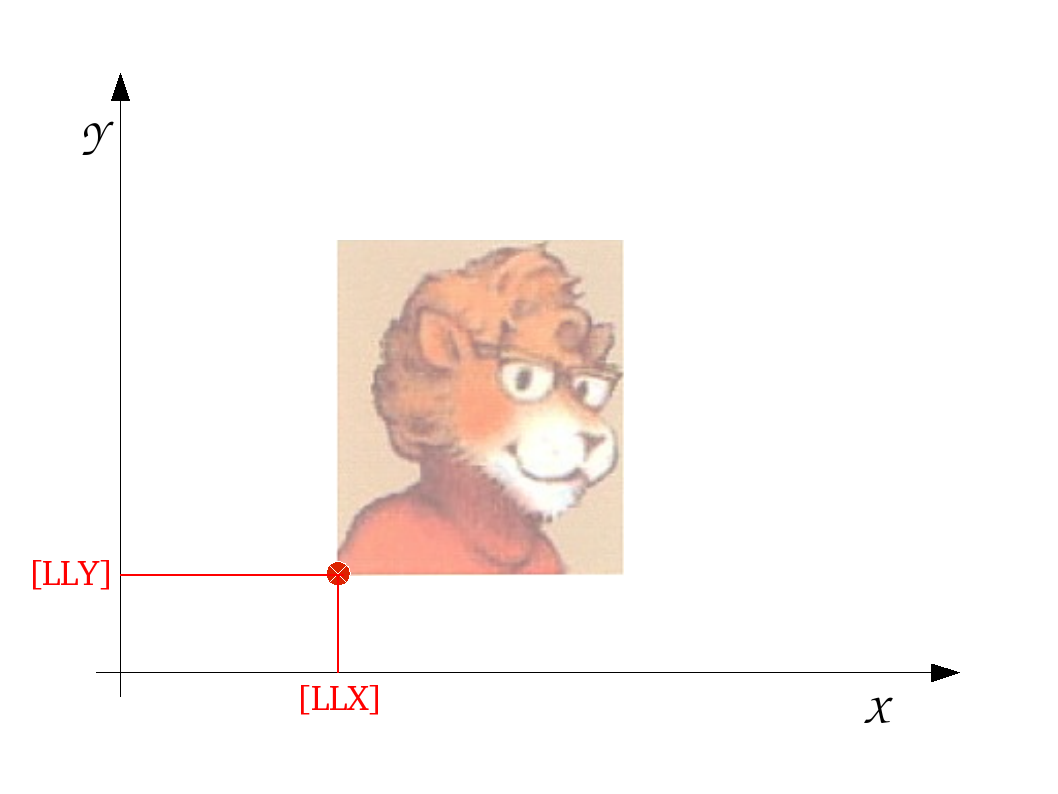
\includegraphics[width=.6\textwidth]{boundingbox_6}
	\end{center}
	\begin{LaTeXcode}
		\\includegraphics[bb= \alert{LLX LLY} URX URY]\{lion\}
	\end{LaTeXcode}
\end{frame}
%-----------------------------------------------------------
%--------------------------------------------------- SLIDE -
\begin{frame}
  \frametitle{\textit{Boundingbox}}
	\begin{center}
	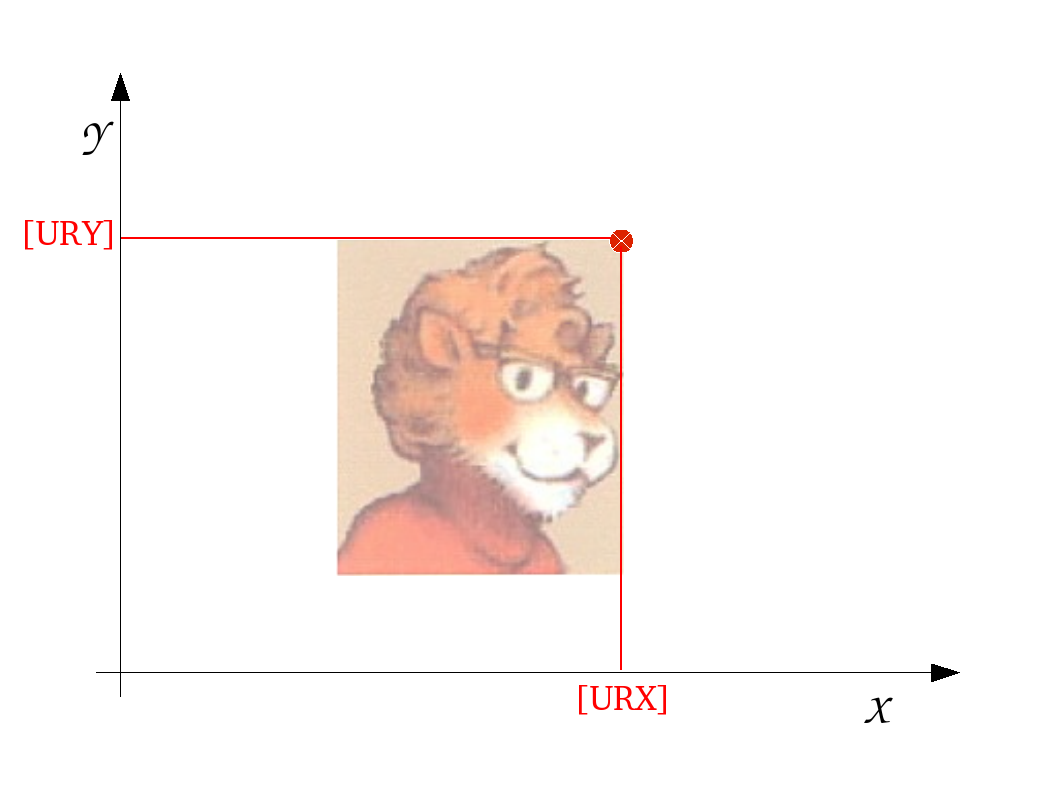
\includegraphics[width=.6\textwidth]{boundingbox_7}
	\end{center}
	\begin{LaTeXcode}
		\\includegraphics[bb= LLX LLY \alert{URX URY}]\{lion\}
	\end{LaTeXcode}
\end{frame}
%-----------------------------------------------------------
%--------------------------------------------------- SLIDE -
\begin{frame}
  \frametitle{\textit{Boundingbox}}
	\begin{LaTeXcode}
		\\fbox\{\\includegraphics\alert{[bb= 0 0 100 120]}\{lion\}\}
	\end{LaTeXcode}
	\begin{center}
	\fbox{
\includegraphics[bb= 0 0 100 120]{lion}}
	\end{center}
	In questa immagine i boundingbox corrispondono con le sue dimensioni (in punti)
\end{frame}
%-----------------------------------------------------------
%--------------------------------------------------- SLIDE -
\begin{frame}
  \frametitle{\textsl{Boundingbox}}
	\begin{LaTeXcode}
		\\includegraphics[bb= 0 0 100 \alert{200}]\{lion\}
	\end{LaTeXcode}
	\begin{center}
		
\includegraphics[bb= 0 0 100 200]{lion}
	\end{center}
\end{frame}
%-----------------------------------------------------------
%--------------------------------------------------- SLIDE -
\begin{frame}
  \frametitle{\textsl{Boundingbox}}
	\begin{LaTeXcode}
		\alert{\\fbox\{}\\includegraphics[bb= 0 0 100 \alert{200}]\{lion\}\alert{\}}
	\end{LaTeXcode}
	\begin{center}
		\fbox{
\includegraphics[bb= 0 0 100 200]{lion}}
	\end{center}
\end{frame}
%-----------------------------------------------------------
%--------------------------------------------------- SLIDE -

\begin{frame}
  \frametitle{\textsl{Boundingbox}}
	\begin{LaTeXcode}
		\\fbox\{\\includegraphics[bb= 0 0 100 \alert{50}]\{lion\}\}
	\end{LaTeXcode}
	\begin{center}
		\fbox{
\includegraphics[bb= 0 0 100 50]{lion}}
	\end{center}
\end{frame}
%-----------------------------------------------------------
%--------------------------------------------------- SLIDE -
\begin{frame}
  \frametitle{\textsl{Boundingbox}}
	\begin{LaTeXcode}
		\\fbox\{\\includegraphics[bb= 0 0 100 50, \alert{clip}]\{lion\}\}
	\end{LaTeXcode}
	\begin{center}
		\fbox{
\includegraphics[bb= 0 0 100 50,clip]{lion}}
	\end{center}
\end{frame}
%-----------------------------------------------------------
%--------------------------------------------------- SLIDE -
\begin{frame}
  \frametitle{\textit{Boundingbox} negativi}
	\begin{LaTeXcode}
		\\fbox\{\\includegraphics\alert{[bb= -50 -50 100 120]}\{lion\}\}
	\end{LaTeXcode}
	\begin{center}
	\fbox{
\includegraphics[bb= -50 -50 100 120]{lion}}
	\end{center}
\end{frame}
%-----------------------------------------------------------
%--------------------------------------------------- SLIDE -
\begin{frame}
  \frametitle{\textit{Boundingbox}}
	\begin{LaTeXcode}
		\\fbox\{\\includegraphics\alert{[bb= 0 0 100 120, scale=.5]}\n
		\{lion\}\}
	\end{LaTeXcode}
	\begin{center}
		\fbox{
\includegraphics[bb= 0 0 100 120, scale=.5]{lion}}
	\end{center}
\end{frame}
%-----------------------------------------------------------
%--------------------------------------------------- SLIDE -
\begin{frame}
  \frametitle{Un esempio vale pi\`u di mille figure}
	\begin{center}
		\alert{\texttt{esempio\_4\_2.tex}}
	\end{center}
\end{frame}

%-----------------------------------------------------------
%---------------------------------------------- SUBSECTION -
\subsection{Ambiente figure}
%-----------------------------------------------------------
%--------------------------------------------------- SLIDE -
\begin{frame}
  \frametitle{A che punto siamo}
  \tableofcontents[currentsection,currentsubsection]
\end{frame}
%-----------------------------------------------------------
%--------------------------------------------------- SLIDE -
\begin{frame}
  \frametitle{L'ambiente \texttt{figure}}
	\begin{LaTeXcode}
		\alert{\\begin\{figure\}[htb]}\n
		\hspace*{5ex}\\centering\n
		\hspace*{5ex}\\includegraphics[scale=.5]\{lion\}\n
		\hspace*{5ex}\\caption\{La mascotte di \TeX\}\\label\{lion\}\n
		\alert{\\end\{figure\}}
	\end{LaTeXcode}
	\begin{figure}[h]
	  \centering
		
\includegraphics[scale=.5]{lion}
		\caption{La mascotte di \TeX}\label{lion}
	\end{figure}
\end{frame}
%-----------------------------------------------------------
%--------------------------------------------------- SLIDE -
\begin{frame}
  \frametitle{Un esempio vale pi\`u di mille figure}
	\begin{center}
		\alert{\texttt{esempio\_4\_3.tex}}
	\end{center}
\end{frame}
%-----------------------------------------------------------
%--------------------------------------------------- SLIDE -
\begin{frame}
  \frametitle{Uso di \texttt{scalebox}}
	\begin{LaTeXcode}
		\\scalebox\{\alert{3}\}\{\\TeX\\ \ non \`e Tex!\}
	\end{LaTeXcode}
	\begin{block}{}
	  \rmfamily
		\scalebox{3}{\TeX\ non \`e Tex!}
	\end{block}
  \bigskip
	\begin{block}{Il bello di \LaTeX}<2->
		Ma non dimentichiamoci che ai matematici (Knuth) piace molto giocare coi numeri
	\end{block}
\end{frame}
%-----------------------------------------------------------
%--------------------------------------------------- SLIDE -
\begin{frame}
  \frametitle{Uso di \texttt{scalebox}}
	\begin{LaTeXcode}
		\\scalebox\{\alert{-3}\}\{\\TeX\\ \ non \`e Tex!\}
	\end{LaTeXcode}
	\begin{LaTeXoutput}
		\scalebox{-3}{\TeX\ non \`e Tex!}
	\end{LaTeXoutput}
\end{frame}
%-----------------------------------------------------------
%--------------------------------------------------- SLIDE -
\begin{frame}
  \frametitle{Uso di \texttt{scalebox}}
	\begin{LaTeXcode}
		\\scalebox\{-3\}\alert{[1.5]}\{\\TeX\\ \ non \`e Tex!\}
	\end{LaTeXcode}
	\begin{LaTeXoutput}
		\scalebox{-3}[1.5]{\TeX\ non \`e Tex!}
	\end{LaTeXoutput}
\end{frame}
%-----------------------------------------------------------
%--------------------------------------------------- SLIDE -

\begin{frame}
  \frametitle{Uso di \texttt{reflectbox}}
	\begin{LaTeXcode}
		\\reflectbox\{\\TeX\\ \ non \`e Tex!\}
	\end{LaTeXcode}
	\begin{LaTeXoutput}
		\reflectbox{\TeX\ non \`e Tex!}
	\end{LaTeXoutput}
\end{frame}
%-----------------------------------------------------------
%--------------------------------------------------- SLIDE -
\begin{frame}
  \frametitle{Usandoli entrambi\dots}
	\begin{LaTeXcode}
		\\reflectbox\{\\scalebox\{-3\}\{\\TeX\\ \ non \`e Tex!\}\}
	\end{LaTeXcode}
	\begin{LaTeXoutput}
		\reflectbox{\scalebox{-3}{\TeX\ non \`e Tex!}}
	\end{LaTeXoutput}
\end{frame}
%-----------------------------------------------------------
%--------------------------------------------------- SLIDE -
\begin{frame}
  \frametitle{Uso di \texttt{rotating}}
	\wheel{fatelo con Word!}
\end{frame}
%-----------------------------------------------------------
%--------------------------------------------------- SLIDE -
\begin{frame}
  \frametitle{Uso di \texttt{scalebox}}
	\begin{LaTeXcode}
		\\scalebox\{-1\}\{\\includegraphics\{lion\}\}
	\end{LaTeXcode}
	\begin{center}
		\scalebox{-1}{
\includegraphics{lion}}
	\end{center}
\end{frame}
%-----------------------------------------------------------
%--------------------------------------------------- SLIDE -
\begin{frame}
  \frametitle{Uso di \texttt{reflectbox}}
	\begin{LaTeXcode}
		\\reflectbox\{\\includegraphics\{lion\}\}
	\end{LaTeXcode}
	\begin{center}
		\reflectbox{
\includegraphics{lion}}
	\end{center}
\end{frame}
%-----------------------------------------------------------
%---------------------------------------------- SUBSECTION -
\subsection{Ambiente picture}
%-----------------------------------------------------------
%--------------------------------------------------- SLIDE -
\begin{frame}
  \frametitle{A che punto siamo}
  \tableofcontents[currentsection,currentsubsection]
\end{frame}
%-----------------------------------------------------------
%--------------------------------------------------- SLIDE -
\begin{frame}
  \frametitle{Produrre grafici con \LaTeX}
	\LaTeX\ prevede la possibilit\`a di disegnare grafici di eccellente qualit\`a. Questa procedura tuttavia non \`e di immediata esecuzione e richiede un approfondimento che trascende gli obiettivi del corso.\newline

  \medskip
	Segue esempio delle potenzialit\`a offerte dalla metodica 
\end{frame}
%-----------------------------------------------------------
%--------------------------------------------------- SLIDE -
\begin{frame}
  \frametitle{Produrre grafici con \LaTeX}
	\begin{LaTeXcode}
		\small
		\\setlength\{\\unitlength\}\{0.15mm\}\n
		\\begin\{picture\}(220,140)(-25,0)\n
		\hspace*{5ex}\\put(0,0)\{\\thicklines \\framebox(100,100)\{\}\}\n
		\hspace*{5ex}\\put(-1.5,105)\{\\line(0,1)\{16\}\}\n
		\hspace*{5ex}\\put(101.2,105)\{\\line(0,1)\{16\}\}\n
		\hspace*{5ex}\\put(105,101.2)\{\\line(1,0)\{16\}\}\n
		\hspace*{5ex}\\put(105,-1.5)\{\\line(1,0)\{16\}\}\n
		\hspace*{5ex}\\put(50,113)\{\\vector(1,0)\{50\}\}\n
		\hspace*{5ex}\\put(50,113)\{\\vector(-1,0)\{50\}\}\n
		\hspace*{5ex}\\put(113,50)\{\\vector(0,1)\{50\}\}\n
		\hspace*{5ex}\\put(113,50)\{\\vector(0,-1)\{50\}\}\n
		\hspace*{5ex}\\put(50,126)\{\\scriptsize \\makebox(0,0)\{\$x\$\}\}\n
		\hspace*{5ex}\\put(126,50)\{\\scriptsize \\makebox(0,0)\{\$x\$\}\}\n
		\hspace*{5ex}\\put(190,50)\{\\small \$\\textrm\{Area\}= x\textasciitilde2\$\}\n
		\\end\{picture\}
	\end{LaTeXcode}
\end{frame}
%-----------------------------------------------------------
%--------------------------------------------------- SLIDE -
\begin{frame}
  \frametitle{Produrre grafici con \LaTeX}
	\begin{LaTeXoutput}
	  \centering
		\setlength{\unitlength}{0.15mm}
		\begin{picture}(220,140)(-25,0)
			\put(0,0){\thicklines \framebox(100,100){}}
			\put(-1.5,105){\line(0,1){16}}
			\put(101.2,105){\line(0,1){16}}
			\put(105,101.2){\line(1,0){16}}
			\put(105,-1.5){\line(1,0){16}}
			\put(50,113){\vector(1,0){50}}
			\put(50,113){\vector(-1,0){50}}
			\put(113,50){\vector(0,1){50}}
			\put(113,50){\vector(0,-1){50}}
			\put(50,126){\scriptsize \makebox(0,0){$x$}}
			\put(126,50){\scriptsize \makebox(0,0){$x$}}
			\put(190,50){\small $\textrm{Area}= x^2$}
		\end{picture}
	\end{LaTeXoutput}
  \onslide<2->
	\begin{block}{Il bello di \LaTeX}
		L'uso di programmi come Gnuplot o Xfig riducono drasticamente i tempi di esecuzione, permettendo di ottenere un output scritto direttamente in codice \LaTeX. 
	\end{block}
\end{frame}
%-----------------------------------------------------------
%--------------------------------------------------- SLIDE -
\begin{frame}
  \frametitle{Produrre grafici con \texttt{Sketch}}
	  \centering
		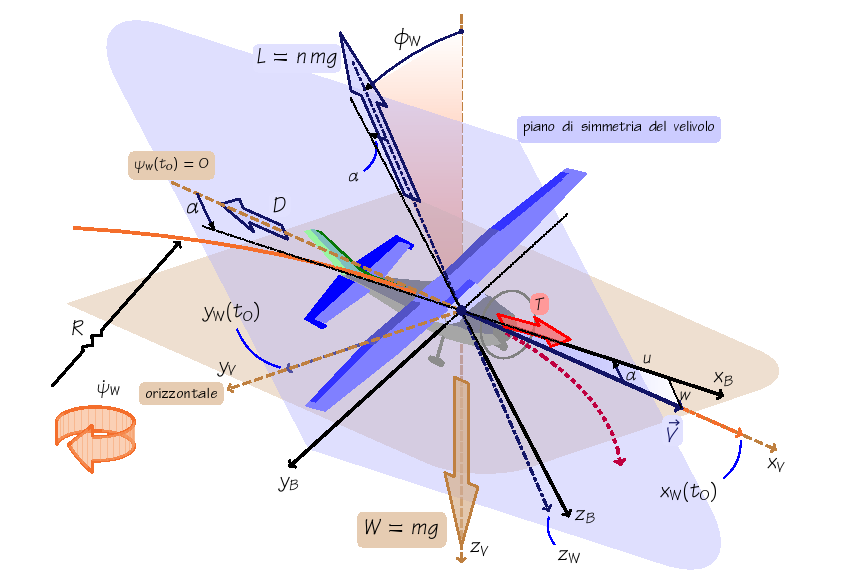
\includegraphics[height=.8\textheight]{tikz}
\end{frame}
%-----------------------------------------------------------
%--------------------------------------------------- SLIDE -
\begin{frame}
  \frametitle{Un esempio vale pi\`u di mille figure}
	\begin{center}
		\alert{\texttt{esempio\_4\_4.tex}}\\
		\alert{\texttt{figura\_1.fig}}
	\end{center}
\end{frame}
%-----------------------------------------------------------
%------------------------------------------------- SECTION -
\section{Videoproiezioni}
%-----------------------------------------------------------
%---------------------------------------------- SUBSECTION -
\subsection[Linee guida]{Linee guida per le videoproiezioni}
%-----------------------------------------------------------
%--------------------------------------------------- SLIDE -
\begin{frame}
  \frametitle{A che punto siamo}
  \tableofcontents[currentsection,currentsubsection]
\end{frame}
%-----------------------------------------------------------
%--------------------------------------------------- SLIDE -
\begin{frame}
  \frametitle{Videoproiezioni}
	\LaTeX\ prevede la possibilit\`a di creare delle presentazioni a video (\textit{slides}) con eccellenti caratteristiche di funzionalit\`a e gradevolezza\\
  \bigskip
	Le Classi di \LaTeX\ per videoproiezioni sono:
	\begin{itemize}
		\item Beamer (argomento di questa lezione)
		\item Pdfscreen
		\item \TeX Power
		\item Prosper
		\item HA-Prosper
		\item Seminar
	\end{itemize}
\end{frame}
%-----------------------------------------------------------
%--------------------------------------------------- SLIDE -
\begin{frame}
  \frametitle{Linee guida per le videoproiezioni}
	Alcune regole per realizzare videoproiezioni:\\
	\begin{itemize}
		\item evitare di presentare pi\`u di una slide a minuto
		\item inserire solo quello che sar\`a adeguatamente commentato
		\item non preparare pi\`u slide di quanto il tempo a disposizione non permetta
	\end{itemize}
  \onslide<2->
	\begin{block}{Attenzione!}
	Le videoproiezioni \emph{non} sono documenti
  \onslide<3->
	\newline
	e questo vale sia per la comunicazione che per la didattica
	\end{block}
\end{frame}
%-----------------------------------------------------------
%--------------------------------------------------- SLIDE -
\begin{frame}
  \frametitle{Linee guida per le videoproiezioni}
	Inoltre\dots
	\begin{itemize}
		\item organizzare la presentazione in sezioni e sottosezioni (mai meno di due e mai pi\`u di quattro) 
		\item usare le animazioni solo se strettamente necessario
		\item usare solo frasi brevi
		\item usare sempre stesso layout per testo e figure
		\item usare dei colori testo/sfondo complementari
		\item evitare caratteri piccoli (``\textit{cos\`i entra pi\`u testo}'')
		\item preferire font sans-serif al \textrm{serif}
		\item evitare il rientro all'inizio della frase
		\item sopratutto: \textit{keep it simple!}
	\end{itemize}
\end{frame}
%-----------------------------------------------------------
%--------------------------------------------------- SLIDE -
\begin{frame}
  \frametitle{Come \textbf{non} presentare}
	\begin{center}
		\alert{\texttt{esempio\_4\_5\_a.ppt}}\\
		\alert{\texttt{esempio\_4\_5\_b.ppt}}\\
		\alert{\texttt{esempio\_4\_5\_c.ppt}}
	\end{center}
\end{frame}
%-----------------------------------------------------------
%---------------------------------------------- SUBSECTION -
\subsection{Sintassi di base}
%-----------------------------------------------------------
%--------------------------------------------------- SLIDE -
\begin{frame}
  \frametitle{A che punto siamo}
  \tableofcontents[currentsection,currentsubsection]
\end{frame}
%-----------------------------------------------------------
%--------------------------------------------------- SLIDE -
\begin{frame}
  \frametitle{Il modello di un documento}
	\begin{LaTeXcode}
		\\documentclass\{\alert{beamer}\}\n
	  \onslide<2->
		\\usetheme\{\alert{<nome-tema>}\}\n
	  \onslide<3>
		\\usepackage[<argomenti-opz>]\{<nome-package>\}\n
	  \onslide<4->
	  \smallskip
		\\begin\{document\}\n
	  \onslide<5->
		\hspace*{5ex}\\begin\{\alert{frame}\}\n
	  \onslide<6->
		\hspace*{10ex}\\frametitle\{\alert{<titolo-slide>}\}\n
		\hspace*{15ex}\alert{<testo della slide>}\n
	  \onslide<5->
		\hspace*{5ex}\\end\{\alert{frame}\}\n
	  \onslide<7->
		\hspace*{10ex}\vdots\n
	  \onslide<4->
		\smallskip
		\\end\{document\}
	\end{LaTeXcode}
\end{frame}
%-----------------------------------------------------------
%--------------------------------------------------- SLIDE -
% \begin{frame}
%   \frametitle{Le opzioni di }
% 	\begin{LaTeXcode}
% 		\\documentclass[\alert{<argomenti-opz>}]\{beamer\}
% 	\end{LaTeXcode}
% 	\begin{itemize}
% 		\item \Lopt{draft}, compila solo una bozza
% 		\item \Lopt{pdftex},
% 		\item \dots
% 	\end{itemize}
% \end{frame}
%-----------------------------------------------------------
%--------------------------------------------------- SLIDE -
\begin{frame}
  \frametitle{La pagina del titolo}
	Nel preambolo:
	\begin{LaTeXcode}
		\\title\{\alert{<titolo-esteso>}\}\n
% 		\\subtitle\{\alert{<sottotitolo>}\}\n
		\\author\{\alert{<nome-autore>}\}\n
% 		\\institute\{\alert{<nome-universit\`a>}\}\n
		\\date\{\alert{<data>}\}
	\end{LaTeXcode}
  \onslide<2->
	Come prima slide:
	\begin{LaTeXcode}
		\\begin\{frame\}\n
		\hspace*{5ex}\alert{\\maketitle}\n
		\\end\{frame\}
	\end{LaTeXcode}
\end{frame}
%-----------------------------------------------------------
%--------------------------------------------------- SLIDE -
\begin{frame}
  \frametitle{Un esempio vale pi\`u di mille slide}
	\begin{center}
		\alert{\texttt{esempio\_4\_6.tex}}
	\end{center}
\end{frame}
%-----------------------------------------------------------
%--------------------------------------------------- SLIDE -
\begin{frame}
  \frametitle{I temi di Beamer}
	\`E possibile modificare il layout della presentazione semplicemente specificando nel preambolo:
	\begin{LaTeXcode}
		\\usetheme\{\alert{<nome-tema>}\}
	\end{LaTeXcode}
	I temi hanno prevalentemente nomi di citt\`a:
	\begin{itemize}
		\item \Lopt{Madrid}
		\item \Lopt{Berkeley}
		\item \Lopt{Goettingen}
		\item \Lopt{Marburg}
		\item \dots
	\end{itemize}
\end{frame}
%-----------------------------------------------------------
%--------------------------------------------------- SLIDE -
\begin{frame}
  \frametitle{I temi interni di Beamer}
	Beamer prevede anche la possibilit\`a di personalizzare l'aspetto degli elenchi puntati e numerati. Nel preambolo va inserito:
	\begin{LaTeXcode}
		\\useinnertheme\{\alert{<nome-tema>}\}
	\end{LaTeXcode}
	Gli schemi di colori hanno prevalentemente nomi delle corrispettive forme geometriche o soluzioni di visualizzazione:
	\begin{itemize}
		\item \Lopt{circles}
		\item \Lopt{rectangles}
		\item \Lopt{rounded}
		\item \Lopt{inmargin}
		\item \dots
	\end{itemize}
\end{frame}
%-----------------------------------------------------------
%--------------------------------------------------- SLIDE -
\begin{frame}
  \frametitle{Schemi di colori}
	\`E possibile scegliere tra diversi schemi di colore
	\begin{LaTeXcode}
		\\usecolortheme\{\alert{<nome-tema>}\}
	\end{LaTeXcode}
	Gli schemi di colori hanno prevalentemente nomi di animali:
	\begin{itemize}
		\item \Lopt{albatross}
		\item \Lopt{crane}
		\item \Lopt{seagull}
		\item \Lopt{whale}
		\item \dots
	\end{itemize}
\end{frame}
%-----------------------------------------------------------
%--------------------------------------------------- SLIDE -
\begin{frame}
  \frametitle{Un esempio vale pi\`u di mille slide}
	\begin{center}
		\alert{\texttt{esempio\_4\_7.tex}}
	\end{center}
\end{frame}
%-----------------------------------------------------------
%--------------------------------------------------- SLIDE -
\begin{frame}
  \frametitle{La pagina dell'indice}
	Analogamente con qualsiasi altro documento l'indice si richiama con il comando \LCmd{tableofcontents} 
	\begin{LaTeXcode}
		\\begin\{frame\}\n
		\\frametitle\{Piano della presentazione\}\n
		\hspace*{5ex}\alert{\\tableofcontents}\n
		\\end\{frame\}
	\end{LaTeXcode}
\end{frame}
%-----------------------------------------------------------
%--------------------------------------------------- SLIDE -
\begin{frame}
  \frametitle{La bibliografia}
	La realizzazione della bibliografia segue schemi gi\`a sperimentati per la realizzazione di un qualunque altro documento
	\begin{LaTeXcode}
		\\begin\{frame\}\n
		\\frametitle\{Bibliografia\}\n
		\hspace*{5ex}\alert{\\begin\{thebibliography\}\{\}}\n
		\hspace*{15ex} \vdots\n
		\hspace*{5ex}\alert{\\end\{thebibliography\}}\n
		\\end\{frame\}
	\end{LaTeXcode}
\end{frame}
%-----------------------------------------------------------
%--------------------------------------------------- SLIDE -
\begin{frame}
  \frametitle{Elenchi numerati}
	Con Beamer \`e possibile far scorrere in successione tutti i punti di una lista
	\begin{LaTeXcode}
		\\begin\{itemize\}\n
		\hspace*{5ex}\\item\alert{<1->} Giovannona Coscialunga\n
		\hspace*{5ex}\\item\alert{<2->} L'Esorciccio\n
		\hspace*{5ex}\\item\alert{<3->} La Polizia s'incazza\n
		\\end\{itemize\}
	\end{LaTeXcode}
  \onslide<2->
	\begin{block}{}
		\begin{itemize}
			\item<3-> Giovannona Coscialunga%
			\item<4-> L'Esorciccio%
			\item<5-> La Polizia s'incazza%
		\end{itemize}
	\end{block}
\end{frame}
%-----------------------------------------------------------
%--------------------------------------------------- SLIDE -
\begin{frame}
  \frametitle{Elenchi numerati}
	Un metodo alternativo \`e il seguente:
	\begin{LaTeXcode}
		\\begin\{itemize\}\alert{<+->}\n
		\hspace*{5ex}\\item Giovannona Coscialunga\n
		\hspace*{5ex}\\item L'Esorciccio\n
		\hspace*{5ex}\\item La Polizia s'incazza\n
		\\end\{itemize\}
	\end{LaTeXcode}
\end{frame}
%-----------------------------------------------------------
%--------------------------------------------------- SLIDE -
\begin{frame}
  \frametitle{Elenchi numerati evidenziati}
	Con l'opzione \LCmd[]{<+-| alert@+>} il punto attivo appare evidenziato
	\begin{LaTeXcode}
		\\begin\{itemize\}\alert{[<+-| alert@+>]}\n
		\hspace*{5ex}\\item Giovannona Coscialunga\n
		\hspace*{5ex}\\item L'Esorciccio\n
		\hspace*{5ex}\\item La Polizia s'incazza\n
		\\end\{itemize\}
	\end{LaTeXcode}
  \onslide<2->
	\begin{block}{}
		\begin{itemize}[<+-| alert@+>]
			\item Giovannona Coscalunga
			\item L'Esorciccio
			\item La Polizia s'incazza
		\end{itemize}
	\end{block}
\end{frame}
%-----------------------------------------------------------
%--------------------------------------------------- SLIDE -
\begin{frame}
  \frametitle{Grafici} 
	Per realizzare una sequenza di grafici useremo l'opzione \Lopt{<n>}
	\begin{LaTeXcode}
		\\includegraphics\alert{<1>}\{lion\_1.png\}\n
		\\includegraphics\alert{<2>}\{lion\_2.png\}\n
		\\includegraphics\alert{<3>}\{lion\_3.png\}
	\end{LaTeXcode}
	\begin{LaTeXoutput}
		\includegraphics<1>{lion_1.png}%
		\includegraphics<2>{lion_2.png}%
		\includegraphics<3>{lion_3.png}%
	\end{LaTeXoutput}
\end{frame}
%-----------------------------------------------------------
%--------------------------------------------------- SLIDE -
\begin{frame}
  \frametitle{Grafici} 
	Per realizzare una successione di grafici useremo l'opzione \Lopt{<n->}
	\begin{LaTeXcode}
		\\includegraphics<1\alert{-}>\{lion\_1.png\}\n
		\\includegraphics<2\alert{-}>\{lion\_2.png\}\n
		\\includegraphics<3\alert{-}>\{lion\_3.png\}
	\end{LaTeXcode}
	\begin{LaTeXoutput}
		\includegraphics<1->{lion_1.png}%
		\includegraphics<2->{lion_2.png}%
		\includegraphics<3->{lion_3.png}%
	\end{LaTeXoutput}
\end{frame}
%-----------------------------------------------------------
%--------------------------------------------------- SLIDE -
\begin{frame}
  \frametitle{Dividere in tempi la slide}
	La visualizzazione in pi\`u tempi pu\`o aiutare a seguire la costruzione di un ragionamento logico, \`e saggio tuttavia limitarne l'utilizzo ai soli casi necessari
  \onslide<2->
	\begin{LaTeXcode}
		Petardi, castagnole, scoppiarelli \n
		\hspace*{5ex}\alert{\\onslide<2->}\n
		Raudi, maradone, trictrac
	\end{LaTeXcode}
	\begin{block}{}
		Petardi, castagnole, scoppiarelli\\
		\onslide<3->
		Raudi, maradone, trictrac
	\end{block}
\end{frame}
%-----------------------------------------------------------
%--------------------------------------------------- SLIDE -
\begin{frame}
  \frametitle{Un esempio vale pi\`u di mille slide}
	\begin{center}
		\alert{\texttt{esempio\_4\_8.tex}}
	\end{center}
\end{frame}
%-----------------------------------------------------------
%--------------------------------------------------- SLIDE -
\begin{frame}
  \frametitle{Blocchi orizzontali}
	La divisione in blocchi \`e molto utile per suddividere i contenuti logici di una slide e/o enfatizzare alcuni aspetti
	\begin{LaTeXcode}
		\alert{\\begin\{}block\alert{\}\{\}}\n
			\hspace*{5ex} Le vittorie di Fantaman\n
		\alert{\\end\{}block\alert{\}}
	\end{LaTeXcode}
	\begin{block}{}
		Le vittorie di Fantaman
	\end{block}
  \onslide<2->
	\begin{LaTeXcode}
		\\begin\{block\}\{\alert{Titolo del film}\}\n
			\hspace*{5ex} Goldrake contro Mazzinga\n
		\\end\{block\}
	\end{LaTeXcode}
	\begin{block}{Titolo del film}
		Goldrake contro Mazzinga
	\end{block}
\end{frame}
%-----------------------------------------------------------
%--------------------------------------------------- SLIDE -
\begin{frame}
  \frametitle{Testo in colonne}
	Per suddividere il testo in colonne di usa l'ambiente \LCmd[]{columns}
	\begin{LaTeXcode}
		\\begin\{columns\}\n
	  \onslide<2->
		\hspace*{5ex} \alert{\\column[t]\{.5\\textwidth\}}\n
	  \onslide<3->
		\hspace*{10ex} svolto a sinistra?\n 
	  \onslide<2->
		\hspace*{5ex} \alert{\\column[t]\{.5\\textwidth\}}\n
	  \onslide<3->
		\hspace*{10ex} oppure a destra?\n 
	  \onslide<1->
		\\end\{columns\}	
	\end{LaTeXcode}
  \onslide<4->
  \bigskip
	\begin{columns}
	  \column[t]{.5\textwidth}
		svolto a sinistra?
	  \column[t]{.5\textwidth}
		oppure a destra?
	\end{columns}
\end{frame}
%-----------------------------------------------------------
%--------------------------------------------------- SLIDE -
\begin{frame}
  \frametitle{Blocchi verticali}
	I blocchi orizzontali sono usati per confrontare due oggetti 
	\begin{LaTeXcode}
		\\begin\{columns\}\n
	  \onslide<2->
		\hspace*{5ex}\\column[t]\{.5\\textwidth\}\n
	  \onslide<3->
		\hspace*{10ex}\alert{\\begin\{block\}\{\}}\n
		\hspace*{15ex} Born to kill\n
		\hspace*{10ex}\alert{\\end\{block\}}\n
	  \onslide<2->
		\hspace*{5ex}\\column[t]\{.5\\textwidth\}\n
	  \onslide<3->
		\hspace*{15ex}\vdots\n
	  \onslide<1->
		\\end\{columns\}	
	\end{LaTeXcode}
  \onslide<4->
	\begin{columns}
	  \column[t]{.5\textwidth}
		\begin{block}{}
		Born to kill
		\end{block}
	  \column[t]{.5\textwidth}
		\begin{block}{}
		Salviamo le rondini
		\end{block}
	\end{columns}
\end{frame}
%-----------------------------------------------------------
%--------------------------------------------------- SLIDE -
\begin{frame}
  \frametitle{Blocchi verticali}
	I blocchi orizzontali sono usati per confrontare due oggetti 
	\begin{LaTeXcode}
		\\begin\{columns\}\n
		\hspace*{5ex}\\column[t]\{.5\\textwidth\}\n
		\hspace*{10ex}\\begin\{block\}\{\}\n
		\hspace*{10ex}\alert{\\centering}\n
		\hspace*{15ex} Born to kill\n
		\hspace*{10ex}\\end\{block\}\n
		\hspace*{15ex}\vdots\n
		\\end\{columns\}	
	\end{LaTeXcode}
	\begin{columns}
	  \column[t]{.5\textwidth}
		\begin{block}{}
		\centering
		Born to kill
		\end{block}
	  \column[t]{.5\textwidth}
		\begin{block}{}
		\centering
		Salviamo le rondini
		\end{block}
	\end{columns}
\end{frame}
%-----------------------------------------------------------
%--------------------------------------------------- SLIDE -
\begin{frame}
  \frametitle{Un esempio vale pi\`u di mille slide}
	\begin{center}
		\alert{\texttt{esempio\_4\_9.tex}}
	\end{center}
\end{frame}
%-----------------------------------------------------------
%--------------------------------------------------- SLIDE -
% \begin{frame}
%   \frametitle{Multimedialit\`a}
% 	Per quanto di utilizzo limitato a pochi casi specifici Beamer permette di inserire dei video all'interno della slide
%   \medskip
% 	\begin{LaTeXcode}
% 		\\movie[<opzioni>]\{<poster testo>\}\{<file>\}	
% 	\end{LaTeXcode}
% 	\begin{block}{Attenzione!}
% 		\`E necessario richiamare il pacchetto \LCmd[]{multimedia}	
% 	\end{block}
% \end{frame}
%-----------------------------------------------------------
%--------------------------------------------------- SLIDE -
% % \begin{frame}
% %   \frametitle{Multimedialit\`a}
% % 	\movie[start=1s]{SV Stunts}{SV_stunts.avi}% cambiare please
% % \end{frame}
% -----------------------------------------------------------
% ------------------------------------------------- SECTION -
\section{Come sopravvivere a \LaTeX}
%-----------------------------------------------------------
%--------------------------------------------------- SLIDE -
\begin{frame}
  \frametitle{Abbiamo quasi finito}
  \tableofcontents[currentsection,currentsubsection]
\end{frame}
% -----------------------------------------------------------
% --------------------------------------------------- SLIDE -
\begin{frame}
  \frametitle{Come affrontare (e superare) i problemi}
	Nei vent'anni di \LaTeX\ sono state sviluppate soluzioni in grado di soddisfare le pi\`u impensate esigenze tipografiche. \`E quindi estremamente improbabile che un problema non sia gi\`a stato affrontato e risolto.\\
  \bigskip
	In qualunque difficolt\`a vi troviate sappiate che, a differenza di molti editor WYSIWYG, la soluzione esiste \emph{quasi} sempre (\LaTeX\ non \`e infatti ancora in grado di preparare un caff\'e decente). 
	\begin{center}
		Occorre solo trovarla\dots
	\end{center}
\end{frame}
% -----------------------------------------------------------
% --------------------------------------------------- SLIDE -
\begin{frame}
	\frametitle{Prima di tutto}
	\`E assolutamente indispensabile leggere una guida di base. Tra i tanti testi liberi in rete, quello consigliato \`e:
	\begin{thebibliography}{Wel66}
		\bibitem [BC07]{BECCARI}
			Beccari, Claudio.
			\newblock \textit{Introduzione all'arte della composizione tipografica}.
			\newblock{\small\url{http://www.guit.sssup.it/downloads/GuidaGuIT.pdf}}
	\end{thebibliography}
  \smallskip
	\`E inoltre indispensabile leggere le guide di tutti i pacchetti che
	si utilizzano e consigliabile consultare le guide citate nella
	bibliografia di ogni lezione.\\
  \smallskip
	Oltre ad internet in \url{../texmf/doc/} \`e disponibile tantissima
	documentazione (quella dei pacchetti \`e in \url{../texmf/doc/latex/})
\end{frame}
%-----------------------------------------------------------
%--------------------------------------------------- SLIDE -
\begin{frame}
  \frametitle{Identificare il problema}
	Il \LaTeX\ si presentano due tipi generali di problemi:
	\begin{itemize}
	\item errori di compilazione: si manifestano quando per un errore nel codice il compilatore non riesce a generare l'output
	\item personalizzare il documento: richiede l'istallazione del pacchetto specifico (quale?) o una conoscenza minima del linguaggio a basso livello 
	\end{itemize}
\end{frame}
%-----------------------------------------------------------
%--------------------------------------------------- SLIDE -
\begin{frame}
  \frametitle{Errori di compilazione} 
	\`E assolutamente inevitabile commettere errori di scrittura del codice. Per evitarli e  correggerli \`e opportuno:
	\begin{itemize}
		\item formattare in maniera pulita il codice
		\item leggere sempre il log del compilatore che spesso riporta il numero della riga dell'errore
		\item compilare il documento per sezioni pu\`o aiutare ad individuare l'errore
		\item correggere un errore appena si presenta
	\end{itemize}
\end{frame}
%-----------------------------------------------------------
%--------------------------------------------------- SLIDE -
\begin{frame}
  \frametitle{Personalizzare il documento}
	La ricerca di personalizzazioni di particolari oggetti o dell'intero documento \`e un processo che presto o tardi tutti si trovano ad affrontare. Per trovare lo specifico pacchetto che soddisfa l'esigenza si pu\`o ricorrere alle seguenti risorse:
	\begin{itemize}
	\item ricerca su Sarovar (\url{http://texcatalogue.sarovar.org/})
	\item ricerca su CTAN (\url{http://www.ctan.org/})
	\item forum di \GuIT\  (\url{http://www.guit.sssup.it/forum/})
	\end{itemize}
  \onslide<2->
	\begin{block}{Attenzione!}
		Nel caso dell'ultima soluzione assicuratevi di avere letto la \textit{netiquette} prima di postare un messaggio o una richiesta di aiuto.
	\end{block}
\end{frame}
%-----------------------------------------------------------
%--------------------------------------------------- SLIDE -
\section*{}
\begin{frame}
  \frametitle{Domande e risposte}
\begin{center}
\scalebox{2}{\Huge
$\nabla{\o}_{m}$\raisebox{-5pt}{$\forall$}$^{n}\partial\varepsilon$\rmfamily
?}
\end{center}
\end{frame}
%-----------------------------------------------------------
%--------------------------------------------------- SLIDE -
% \begin{frame}
%   \itshape
% 	\LaTeX, purtroppo, non pu\`o far nulla per rendere migliori i contenuti.
% 	\begin{flushright}\upshape
% 		Rosa Gini
% 	\end{flushright}
% \end{frame}
%-----------------------------------------------------------
%----------------------------------------------------- END -
\end{document}
